%Resume protokol
%kelompok 3 D4 TI-2B 
%Fikri aldi nugraha                  1164038
%Nur Arkhamia Batubara               1164049 
%Miftahul Hasanah                    1164046 
%Si Made Angga Dwitya P              1164053 
%Widary Anggraini Mindo V Siahaan    1164057


\section{Pengenalan Protokol} 
 Suatu standar pertukaran informasi. Komputer dengan system operasi dan software berbeda dapat saling berkomunikasi melalui internet 
 karena pengadopsian protokol. Seperangkat aturan umum (atau bahasa) yang mengijinkan komputer-komputer untuk saling berkomunikasi. 
 Protokol yang standart adalah TCP/IP (Transmission Control Protocol/Internet Protocol). Web menggunakan server protokol HTTP agar 
 komputer dapat mengakses file , melakukan pencetakan, berkomunikasi, dan menyediakan layanan lain bagi user lain dalam jaringan.
 
 \ref{osilayer} 
    \begin{figure}[ht] 
    \centerline{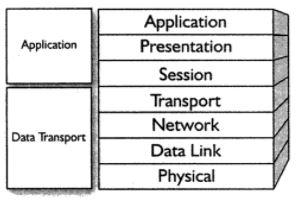
\includegraphics[width=1\textwidth]{figures/osilayer.JPG}} 
    \caption{dua bagian osi layer} 
    \label{osilayer} 
    \end{figure}
 
 \section{Pengertian Protokol}
Protokol merupakan aturan dalam melakukan pengiriman data (berupa blok-blok data) dari sebuah node jaringan ke node jaringan lain.
Protokol merupakan sarana komunikasi antara mesin melalui jaringan yang terstandarisasi. Protokol mengizinkan data untuk ambil bagian dalam transmisi kilat, kemudian ditransmisikan, lalu dikumpulkan kembali sesuai arah dengan perintah yang benar. 
Protokol digunakan untuk mendeteksi kesalahan, tipe kompresi, dan bagaimana receiver (penerima) mengindikasikan bahwa pesan telah diterima. 
 
 \section{Jenis-Jenis Protokol}
Protokol jaringan adalah berbagai protokol yang terdapat dari lapisan  teratas sampai terbawah yang ada dalam sederetan protocol.
Di pandang dari sudut komunikasi data,ada beberapa protokol yang banyak digunakan pada jaringan computer, di antaranya:

 \subsection{TCP/IP}
TCP/IP merupakan protokol standar pada jaringan internet yang tidak tergantung pada jenis computer yang digunakan.
Barangkali perlu dicatat bahwa TCP/IP adalah perlengkapan standar pada sistem operasi Unix dan turunannya.
Saat ini mesin novell,SUN maupun Machintosh sudah dilengkapi protokol standar TCP/IP ini.

Protocol adalah spesifikasi forma yang mendefenisikan prosedur-prosedur yang harus diikuti ketika mengirim dan menerima data (Wermer, 
1996). Protocol mendefenisikan jenis, waktu, urutan dan pengecekan kesalahan yang digunakan dalam jaringan. Transmission control 
protocol/internet protocol (TCP/IP) merupakan protocol untuk mengirim data antar computer pada jaringan. Protocol ini merupakan protocol 
yang digunakan untuk akses internet dan digunakan untuk komunikasi lobal. TCP/IP terdiri atas dua protocol yang terpisah. TCP/IP 
menggunakan pendekatan lapisan (layer) pada saat membangun protocol ini. Dengan adanya pendekatan berlapis ini memungkinkan dibangunnya 
beberaa layanan kecil untuk tugas-tugas khusus.
  
 \subsection{AppleTalk} 
Protokol AppleTalk diciptakan oleh perusahann Apple Computer, diterapkan pada jaringan dengan komputer mesin Apple, yang diperkenalkan 
pada tahun 1985. Protokol ini menduung teknologi milik Apple. Metode akses LocalTalk berfungsi sebaik Ethernet dan Token Ring. Manajemen 
jaringan AppleTalk dan metode akses LocalTalk telah digabungkan ke dalam semua mesin Macintosh dan LaserWriter. Bersama produk lainnya 
dari Apple dan mesin tipe lain, AppleTalk dapat dijalankan di PC, VAX dan workstation UNIX.
